\documentclass[11]{article}
\usepackage{graphicx}
\usepackage{placeins}
\title{Simulating and Reconstructing X-ray Computerized Tomography}
\author{Xiang Gao, Qi Li, Suerfu and Yao Zhou}

\date{\today}

\begin{document}
	\maketitle
	
\begin{abstract}
	We propose as APC524 final project a software that simulates X-ray radio-graph and reconstructs the result information to obtain the cross-sectional images of objects imaged. Since its discovery, X-rays are playing an increasingly important role, both in our lives and in scientific research. One application is tomographic imaging: using the penetrating property of X-rays and a proper reconstruction algorithm to reconstruct cross-sectional images from projection images. As the final project of APC524, we would like to design a software that simulates the imaging and reconstruction processes, at least for simple objects. In the remainder of the proposal, we would like to show how such a project fits into the principles of APC524 and would like to convince such a project is a suitable final project.
\end{abstract}

\section{What is Computerized Tomography?}
	X-ray is a type of penetrating elecromagnetic radiation. X-ray images can be obtained by recording the X-ray intensity after X-ray passes through an object. Such image is called X-ray radio-graph. Considering the attenuation of X-ray in different objects, the intensity at each point is essentially a line integral of attenuation coefficient. Therefore, light region will appear as having large X-ray intensity, while dense object will show up with small X-ray intensity.\\ \\
	The questions is: if we have X-ray density images taken from different angles, do we have enough information to reconstruct how the object looks like in the high dimension. To rephrase, can we reconstruct a 2D(3D) object from many 1D(2D) images? This is the subject of tomographic image reconstruction, and was first mathematically proven possible by Johann Radon. Later, Godfrey Hounsfield built an X-ray scanner, with which he demonstrated the possibility of reconstructing cross-sectional images of daily objects, for which he was awarded a Nobel prize for physiology. With the aid of modern high-performance computers, tomographic image reconstruction can be handled much faster than the times of Hounsfield. It also explains the name X-ray Computerized Tomography.
\\ \\
	In this project, we propose to develop a software that illustrates the X-ray tomographic reconstruction process, and potentially tests the performance of different algorithms.  

\section{What is the structure of the project?}
At this stage, the blueprint of the project consists of: Geometry construction, X-ray simulation, tomographic image reconstruction, and image processing. Below we explain each module. The flow of the program is also shown in Fig.~\ref{program_flow}.
	\begin{figure}
	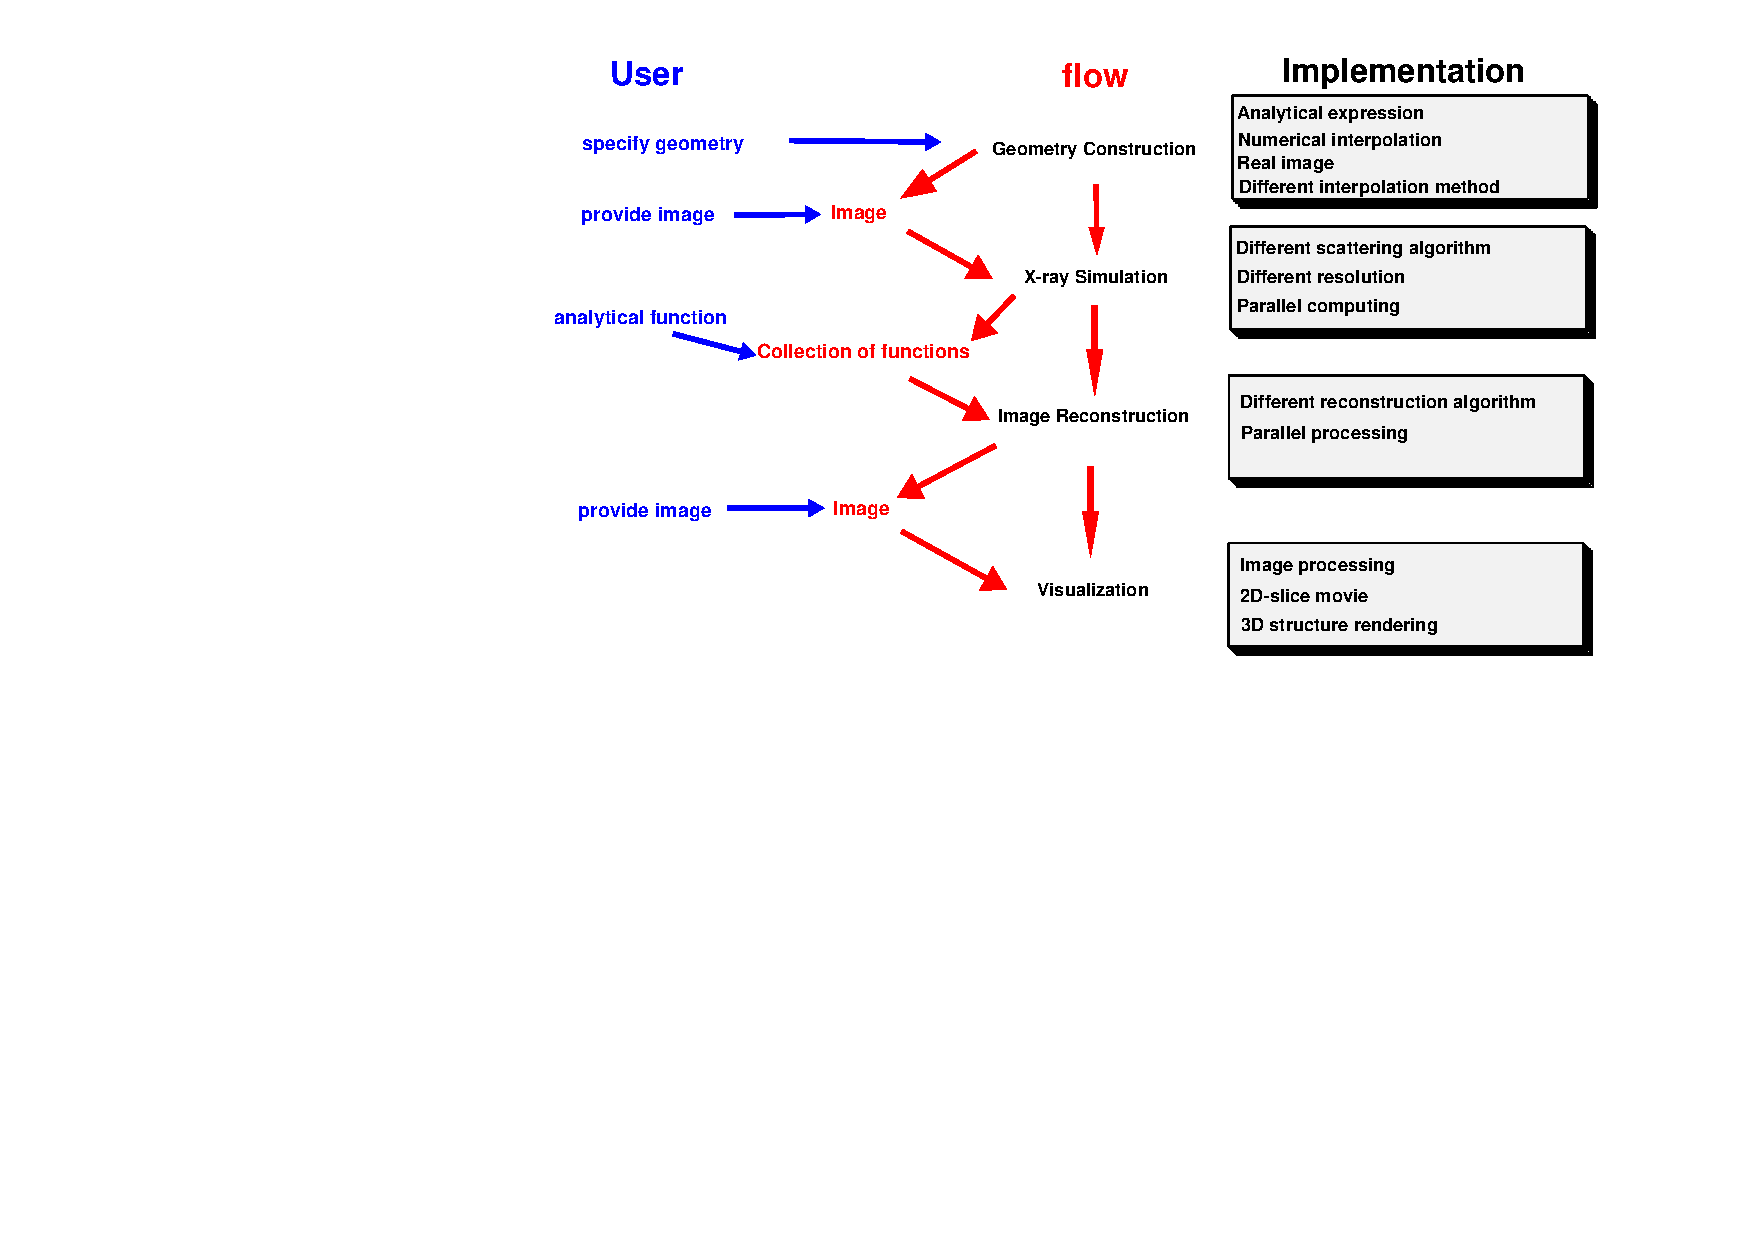
\includegraphics[scale=0.7]{flow}
	\centering
	\caption{Figure showing how user interacts with the program. The left column shows how user interacts with the program, and the central column shows the flow of the program. The right column is different potential implementations at each stages.}
	\label{program_flow}
	\end{figure}
	\subsection{Geometry Construction:}
		This module constructs geometric objects for X-ray simulation. At the beginning, the geometric objects can be as simple as a sphere inside a cube, of different material/X-ray attenuation coefficient. This geometric information is passed along to X-ray simulations.

	\subsection{X-ray Simulation:}
		This module takes the geometric information and produces simulated X-ray projection images from each angle. This information is passed along to tomographic image reconstruction.

	\subsection{Tomographic Image Reconstruction:}
		From the X-ray projection image and the angular information, this module uses different algorithm to reconstruct the tomographic image from the projection images. Different algorithms can be implemented here, such as radon-transform or filtered back-projection. The result is passed along to image processing module.

	\subsection{Image Visualization:}
		This module takes reconstructed tomographic images as the input, and does operations on the images. Potential operations can include various smoothing/filtering processes, making a movie of the image slice moving through the object, or if time allows, combining different cross-sectional images to form a 3D image. 
	\subsection{Automated Tests:}
		Since in each module, the physics is well-understood, and we know exactly what should happen. It would be ideal to devise several test cases to test the accuracy and correctness of the program.\\ Tomographic image reconstruction can be applied both in 2D and 3D. As a start-up, we can work and test on 2D cases, and by designing a good interface, we can extend the functionality of the software to 3D.

\section{How does the interface look like?}
	There should be two classes at minimum: image and image container.\\ Images are the direct product of geometry generator and X-ray simulators. Let's think about the process of X-ray simulations: all X-ray simulation needs to know is given a spatial point, the (electronic) density at that point. Once known, X-ray simulators would be able to perform line integrals along every line. Therefore, the interface of the image object is a method that gives functional value corresponding to a particular point. As for whether this should be done analytically or numerically, or by what kind of interpolations, how many data points the image has, should be hidden in the implementation. \\
	X-ray simulator would take this geometric image and return the line integral along parallel lines at the same angle (see Fig.~\ref{line_integral}). Then the object is a function with the parallel displacement being the independent variable. The X-ray simulator should pass a collection of such object(function) along different angles to the reconstruction module. Such collection of 1D functions should be contained in a container class. So we have the main structure of the two important interfaces.
	\begin{itemize}
		\item[Image]
			Image has a method that returns the function values at different input points. Since the software should work on 2D and 3D cases, it should contain data of it's physical dimensionality as well as the range of index and/or physical boundaries.
		\item[Image Container]
			Image container should return line-integrated functions corresponding to different angles. At minimum, it should contain these functions and corresponding angles.
	\end{itemize}

	\begin{figure}{ht!}
	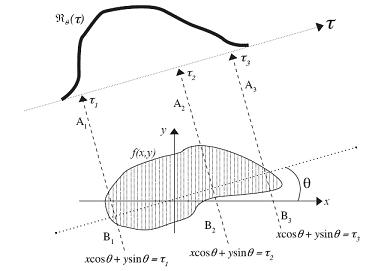
\includegraphics[scale=0.8]{line_integral}
	\centering
	\caption{From a 2D scalar field, obtain line integrals along different lines with the same angle\cite{line_integral}.}\label{line_integral}
	\end{figure}


\section{Why CT for final project?}
	In this section, we would like to discuss why we chose X-ray simulation and reconstruction as our final project.
	\subsection{Educational Purpose}
		Given that all members are from different departments, a project that none of us are familiar with in research would help promote our own knowledge as a learner. It also gives us a chance to dive into a research field of great importance yet possibly less relevance in future research areas of the group members, thus giving us a platform to start from scratch with equal contributions. Unlike some research topics, with fairly straight-forward explanation and demonstration, X-ray CT is easy to understand and appreciate for typical graduate level students, which makes the project particularly suitable for presentation and demonstration.
	
\subsection{Designing to an Interface}
	One important principle we learned in the course is programming to an interface. In the above mentioned structure of the project, it is clear that each module works independently, and connects to each other through an interface or a protocol.\\ For example, the geometry module can construct different geometric objects, as long as the output is to an interface that X-ray simulation module can understand. 	The X-ray simulation module can simulate objects with different X-ray intensity and scattering, and can even load a real medical X-ray image. In either case, the output is to the interface between X-ray simulation and image reconstruction module. The image reconstruction module can call different algorithms through an interface to reconstruct the image.

\subsection{Modular Design for a Team}
	Each module is completely decoupled from each other. So each team member can work on different modules simultaneously without complex dependencies. The project could be easily managed via a git repository. 

\subsection{Automated Tests}
	Each module can come with its own automated tests. And because we are reconstructing simulated objects, at each step we know if the right result has been obtained. For example, in the geometry construction, it is easy to check if the right geometry has been constructed by specifying relatively simple set-ups. The X-ray simulation can take a simple geometry, such as a sphere in a cube, to produce the X-ray image and compare with expectated result. The image reconstruction module can reconstruct with known analytical density plots to see if the right analytical image can be obtained. After each module has passed its own tests and simulation tests, we can potentially try to reconstruct real data from, for example medical X-ray.

\subsection{Parallel Computing}
	Since in tomographic imaging, we need information from multiple angles, the simulation of X-ray projection imaging is by its nature a parallel process. We can exploit this feature by parallel computing. Some reconstruction algorithm, such as Radon transform, can be potentially made parallel as well, since it is a two dimensional integral.

\subsection{Multi-Language}
	Each module communicates through data and interfaces, each module can be potentially implemented in different languages. For example, image reconstruction module involves heavy calculations, therefore Fortran, C and C++ are suitable; however in the geometry and image presentation involves graphics and even movies, a high-level language with many convenient libraries (Python, MATLAB) would be convenient. This can also provide us with a chance to programme in a different language.

\subsection{Feasibility}
	CT reconstruction is a relatively mature field in industry and academia, with many literature and resources available. Faculty and students in astronomy department are also skilled in image processing. Even we encounter difficulties, we believe we can find ample resources for help. Besides, the physics of CT reconstruction is well defined: we will not be constrained by the inherent difficulties in some situations (e.g. traditional molecular dynamics fail at phase transition, or solving chaotic systems), and no complicated algorithm is involved in this project. Nevertheless, this project will potentially demonstrate the key concepts and main ideas of scientific software engineering such as programming to an interface, efficiency and portability.
	

\subsection{Task Designation}
Since we have divided the program into four parts, we would like to designate the task according to these parts. Xiang and Qi will collaborate on geometry construction and X-ray simulation parts. Surfu will be in charge of tomographic image reconstruction. Yao will work on image processing. Since we have designed the interface and decided on the input and output for each component of the program, we can work separately without waiting for other parts to be done.

\section{Task Assignment and External Libraries}
Xiang Gao and Qi Li will be responsible for the geometry construction and X-ray simulations. Suerfu will be responsible for image reconstructions and Yao Zhou will be responsible for visualization. The programming language would be C/C++ combined with Python, except visualization, for which either Python or Matlab will be heavily used. Upon further research, geometry libraries might be referenced in the geometry construction part. In image processing, if matrix methods are incorporated, eigen library would be used as well.\\
Based on the initial discussion, at least X-ray simulation and image processing will be implemented parallel. Note that the details such as external libraries might be subject to changes as more information  and resources become available. 

\section{Timeline}
\begin{itemize}
\item[1] By the end of Thanksgiving, we are planning to finish designing the interface, which will mainly consists of four parts.\\
\item[2] By the end of the semester, we are planning to have the $\alpha$ version ready, which will consist of the skeletons of the four parts. Starting from a simple geometry (probably a two-dimensional object), we will design each component. Without digging into the details of algorithm and optimizing performance of the code, we would like to make sure that the interface is working well. 
\item[3] By the end of winter break, we are plannin to have the $\beta$ version ready. It will be an extended version of $\alpha$. Different alogorithms, complex object shapes and better visualizations will be the main focus of this version.
\end{itemize}
	
\section{Conclusion}
Our project, Simulating and Reconstructing X-ray Tomographic Images, appeals to the general audience with diverse backgrounds. The problem has relatively well-defined modules and interfaces. The process is parallel in nature, allowing better use of computational resources. At each step, simple tests can be implemented to make sure the program is doing the right thing. Because of its modular nature, multiple programming languages can be combined to facilitate the entire project. And most importantly, APC524 is \textbf{not} a course on algorithm; all parts of the project involves only relatively simple computations, such as computing line integrals or two dimensional integrals, fourier-transforms and multi-dimensional array manipulations, yet the physics and mathematics behind the process is ubiquitous and profound. We consider this proposed project as one which integrates various aspects of good practices of programming that we have learned in this course. Therefore, we propose "Simulating and Reconstructing X-ray Tomographic Images" as our final project for APC524. We would greatly appreciate any comment/suggestions! 

\begin{thebibliography}{9}
\bibitem{line_integral}
http://www.mindef.gov.sg/content/imindef/publications/pointer/journals/ 2008/v34n1/techedge.html
\end{thebibliography}
\end{document}
